\documentclass[14pt]{beamer}

\mode<presentation> {
\usetheme{Madrid}

% To remove the navigation symbols from the bottom of all slides uncomment next line
\setbeamertemplate{navigation symbols}{} 
\date{}
\title{}
\author{}

%to get rid of footer entirely uncomment next line
\setbeamertemplate{footline}{}
}


\usepackage{geometry}
\usepackage{multirow}
\usepackage{adjustbox}
\usepackage{multicol}
\setlength{\columnsep}{0.1cm}


\usepackage{tikz}
\usetikzlibrary{shapes,backgrounds}

\usepackage{bbding}
\usepackage{rotating}
\usepackage{xcolor}


%\usepackage{tkz-berge} %cool grid
\usepackage{pgfplots} %pics

\usepackage{graphicx} % Allows including images
\usepackage{booktabs} % Allows the use of \toprule, \midrule and \bottomrule in tables
\usepackage{mathtools}

\newcommand {\DS} [1] {${\displaystyle #1}$}
\newcommand {\R}{\mathbb{R}}
\newcommand {\Z}{\mathbb{Z}}
\newcommand {\N}{\mathbb{N}}
\newcommand{\e}{\varepsilon}

\newcommand{\p}{\pause}

% simple environrment for enumerate, easier to read
\setbeamertemplate{enumerate items}[default]

%%%%%%%%%%%%%%%%%%%%%%

% to use colours easily
\definecolor{verde}{rgb}{0, .7, 0} 
\definecolor{rosa}{rgb}{1, 0, 1}  
\definecolor{naranja}{rgb}{1, .5, 0.1} 
\newcommand{\azul}[1]{{\color{blue} #1}}
\newcommand{\rojo}[1]{{\color{red} #1}}
\newcommand{\verde}[1]{{\color{verde} #1}}
\newcommand{\rosa}[1]{{\color{rosa} #1}}
\newcommand{\naranja}[1]{{\color{naranja} #1}}
\newcommand{\violeta}[1]{{\color{violet} #1}}
 
% box in red and blue in math and outside of math
\newcommand{\cajar}[1]{\boxed{\mbox{\rojo{ #1}}}}
\newcommand{\majar}[1]{\boxed{\rojo{ #1}}}
\newcommand{\cajab}[1]{\boxed{\mbox{\azul{ #1}}}}
\newcommand{\majab}[1]{\boxed{\azul{ #1}}}
 
\newcommand{\setsize}[1]{\fontsize{#1}{#1}\selectfont} %allows you to change the font size. The default size of this document is 14. To change the font size of the whole slide, place this at the beginning of the slide. To change the size of only a portion of the text to size 12, you can do the following { \setsize{12} Your text. }.

\setbeamerfont{frametitle}{size=\setsize{15}}
\setbeamerfont{block title}{size=\setsize{14}}

\newcommand{\smallerfont}{\setsize{13}} %place this at the beginning of a slide to set the font size of the entire slide to 13.

%===========================
% Preamble just for this file
%===========================


\newcommand{\erf}{\operatorname{erf}}
\newcommand{\vv}{\vspace{.2cm}}

%===================================================
\begin{document}
%===================================================

%----------------------------------------------------------------------------------------
%	Integration by substitution
%----------------------------------------------------------------------------------------
%------------------------------
\begin{frame}[t]
\frametitle{Warm up}

Calculate
	$$
		\int \frac{\sin \sqrt{x}}{\sqrt{x}} \, dx
	$$

\emph{Hint:}  Use the substitution \DS{u=\sqrt{x}}.

\end{frame}

%------------------------------
\begin{frame}[t]
\frametitle{Computation practice: integration by substitution}

Use substitutions to compute:
\begin{multicols}{2}
	\begin{enumerate}
		\item \DS{\int \frac{\sin \sqrt{x}}{\sqrt{x}} dx}
		\vv
		\item  \DS{ \int e^x \cos \left(e^x \right) dx }
		\vv
		\item  \DS{ \int \cot x \, dx }
		\vv
		\item  \DS{ \int x^2 \sqrt{x+1} \, dx }
		\vv
\p
		\item \DS{\int \frac{e^{2x}}{\sqrt{e^x + 1}} \, dx}
		\vv
		\item \DS{\int \frac{\left( \ln \ln x \right)^2}{ x \ln x} \, dx}
		\vv
		\item \DS{\int x e^{-x^2} \, dx}
		\vv
		\item \DS{\int e^{-x^2} \, dx}
		\vv
	\end{enumerate}
\end{multicols}

\end{frame}
%------------------------------
\begin{frame}
\smallerfont
\frametitle{Definite integral via substitution}

This final answer is right, but the write-up is WRONG.  Why?
\vfill

Calculate \DS{I = \int_0^2 \sqrt{x^3+1} \; x^2 dx}
\begin{block}{Wrong answer}
Substitution:  \DS{u = x^3+1, \; du=3x^2 dx}.
\begin{align*}
	I \; & = \; 
		 \frac{1}{3} \int_0^2   \sqrt{x^3+1} \; (3x^2 dx) 
	 &&=  \;	
		  \frac{1}{3} \int_0^2   u^{1/2}  \; du
	\\ &=  \;
		\frac{1}{3} \; \frac{2}{3}  \; \left. u^{3/2}  \right\vert_0^2
	&& = \; 
		 \left. \frac{1}{9} \left(x^3+1\right)^{2/3}     \right\vert_0^2	
	\\ &=  \;
		 \frac{2}{9} \left( 2^3 + 1 \right)^{3/2} - \frac{2}{9} \left( 0 + 1\right)^{3/2}  
	&&= \; \frac{52}{9}
\end{align*}
\end{block}

\end{frame}
%------------------------------
\begin{frame}[t]
\smallerfont
\frametitle{Integral of products of $\sin$ and $\cos$}
We want to compute
\vspace{-.5cm}
	$$
		I = \int \sin^3 x \cos^2 x \, dx
	$$

\begin{enumerate}
	\item  Attempt the substitution \DS{u = \sin x}
	\item  Attempt the substitution \DS{u = \cos x}
	\item  One worked better than the other.  Which one?  Why? \\ 
	  Finish the problem.
\p
	\item  Assume we want to compute
		$$
			\int \sin^{n} x \cos^{m} x \, dx
		$$
		When will the substitution \DS{u = \sin x} be helpful? \\
		When will the substitution \DS{u = \cos x} be helpful?
\end{enumerate}

\end{frame}
%------------------------------
\begin{frame}[t]
\smallerfont
\frametitle{Odd functions}

\begin{block}{Theorem}
Let $f$ be a continuous function.  Let $a >0$.  IF $f$ is odd, THEN
	$$
		\int_{-a}^{a} f(x) dx = 0
	$$
\end{block}

\p

\begin{enumerate}
	\item  Write down the definition of ``odd function".
	\item  Draw a picture to interpret the theorem geometrically.
	\item  Prove the theorem!
	
		\emph{Hint:}  Write the integral as sum of two pieces.  Use a substitution to show that one of the two pieces equals minus the other.
\end{enumerate}

\end{frame}
%------------------------------
%----------------------------------------------------------------------------------------
%	Integration by parts
%----------------------------------------------------------------------------------------
%------------------------------
\begin{frame}[t]
\frametitle{Computation practice: Integration by parts}

Use integration by parts (possibly in combination with other methods) to compute:
\begin{multicols}{2}
	\begin{enumerate}
		\item  \DS{ \int x e^{-2x} dx }
		\vv
		\item \DS{\int x^2 \sin x \, dx}
		\vv
		\item \DS{\int  \ln x \, dx}
		\vv
		\item \DS{\int  \sin \sqrt{x} \, dx}
		\vv
\p		\item \DS{\int  x \arctan x \, dx}
		\vv
		\item \DS{\int  x^2 \arcsin x \, dx}
		\vv
		\item \DS{\int  e^{\cos x}  \sin^3 x \, dx}
		\vv
		\item \DS{\int  e^{ax} \sin (bx) dx}
		\vv
	\end{enumerate}
\end{multicols}

\end{frame}
%------------------------------
\begin{frame}[t]
\frametitle{Persistence}
Compute
	\begin{multicols}{2}
	\begin{itemize}
		\item \DS{\int_1^e \left( \ln x \right)^3 dx}
\p
\vv
		\item \DS{\int_1^{e} \left( \ln x \right)^{10} dx}
	\end{itemize}
	\end{multicols}
\p
There is a more efficient approach.  Call
	$$
		I_n = \int_1^e \left( \ln x \right)^n dx
	$$
Use integration by parts on $I_n$.  You will get an equation with $I_n$ and $I_{n-1}$.
Now solve the previous questions.

\vfill
\hfill
\href{https://oeis.org/}{\beamergotobutton{OEIS}}

\end{frame}

%------------------------------
\begin{frame}[t]
\frametitle{Integrals from a graph}

\begin{columns}

\begin{column}{.7\textwidth}
\begin{center}
	\only<1>{ 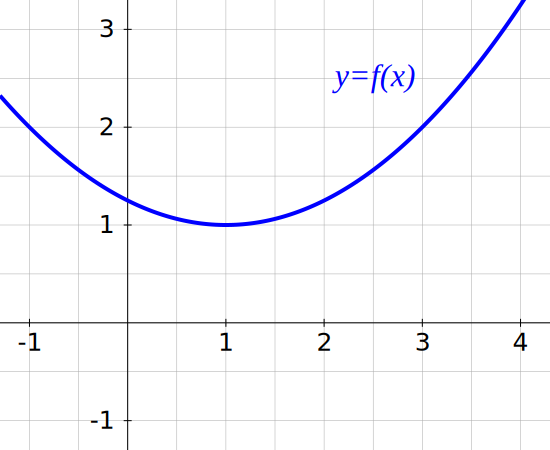
\includegraphics[scale=.4]{G22} }
	\only<2>{ 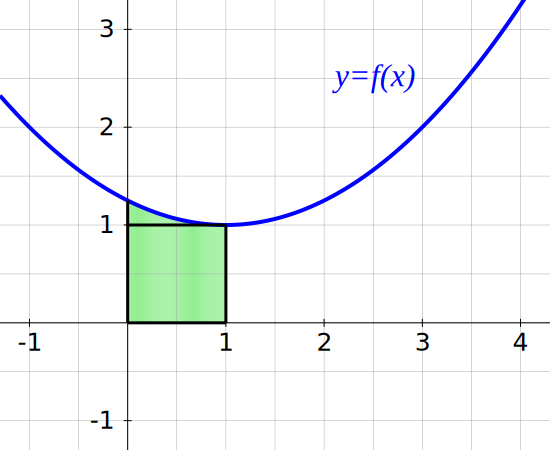
\includegraphics[scale=.4]{G22a} }
	\only<3>{ 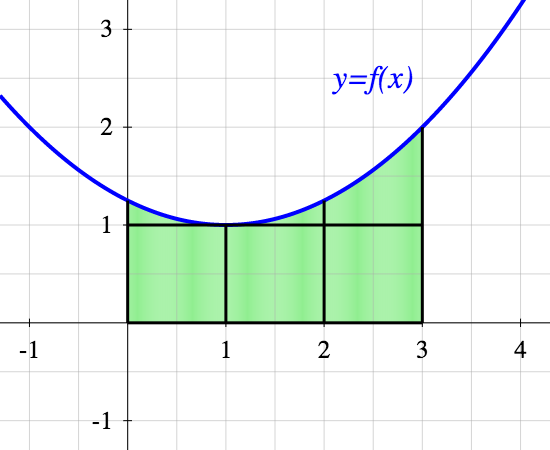
\includegraphics[scale=.4]{G22b} }
\end{center}
\end{column}

\begin{column}{.32\textwidth}
Estimate:
	\begin{enumerate}
		\item  \DS{\int_0^1 f(x) dx}
		\item  \DS{\int_0^1 f'(x) dx}
		\item  \DS{\int_0^3 x \, f'(x) dx}
		\item \DS{\int_0^1 f(3x) dx}
	\end{enumerate}
\end{column}
\end{columns}

\end{frame}
%------------------------------
\begin{frame}[t]
\frametitle{The error function} 

The following function	is tabulated.
	$$
		{\Large E(x) =  \int_0^x e^{-t^2} dt}.
	$$
Write the following quantities in terms of $E$:

\begin{multicols}{2}
	\begin{enumerate}
		\item \DS{\int_1^{2} e^{-t^2} dt}
		
		\vv
		\item \DS{\int_0^x t^2 e^{-t^2} dt}
		
		\vv
		\item  \DS{\int_0^x e^{-2t^2} dt}
		
		\vv
\p		\item  \DS{\int_0^1  e^{-t^2+6t} dt}
		
		\vv
		\item  \DS{\int_{x_1}^{x_2}  e^{-\frac{(t- \mu)^2}{\sigma^2}} dt}

		\vv
		\item  \DS{\int_1^2 \frac{e^{-t}}{\sqrt{t}} dt}
	\end{enumerate}
\end{multicols}

\end{frame}
%------------------------------
\begin{frame}[t]
\frametitle{Exp-trig antiderivative}

We want to compute
	$$
		I = \int e^{ax} \sin (bx) \; dx
	$$
\begin{itemize}
		\item Try once integration by parts choosing \DS{u = e^{ax}}.  Stop.
		\item Go back to $I$.  Now try integration by parts once choosing \DS{u = \sin (bx)} instead.  Stop.
		\item  Look at what you did.  Think.
\end{itemize}

\end{frame}
%------------------------------
%----------------------------------------------------------------------------------------
%	Integration of products of trigonometric functions
%----------------------------------------------------------------------------------------
%------------------------------
\begin{frame}[t]
\smallerfont
\frametitle{Practice: Integrals with trigonometric functions}

Compute the following antiderivatives.  (Once you get them to a form from where you see a path to finish them, even if long, you may stop.)
  
\begin{multicols}{2}
	\begin{enumerate}
		\item  \DS{ \int \sin^{10} x \cos x \ dx }
		\vv
		\item \DS{\int \sin^{10} x \cos^{7} x \, dx}
		\vv
		\item \DS{\int e^{\cos x}  \cos x \sin^3 x \, dx}
		\vv
		\item \DS{\int  \cos^2 x \, dx}
		\vv
		\item \DS{\int  \cos^4x  \, dx}
		\vv
		\item \DS{\int  \csc x \, dx}
		\vv
	\end{enumerate}
\end{multicols}

\vspace{-.5cm}
{\setsize{10}
\begin{block}{ \setsize{12} Useful trig identities}  \vspace{-.5cm}
	\begin{align*} \large
		&\sin^2 x + \cos^2 x = 1
			&
		\sin^2 x &= \frac{1 - \cos (2x)}{2}		
			\\
		&\tan^2 x + 1 = \sec^2 x
			&
		\cos^2 x &= \frac{1 + \cos (2x)}{2}
	\end{align*}
\end{block}
}

\end{frame}
%------------------------------
\begin{frame}[t]
\frametitle{Integral of products of secant and tangent}

To integrate
	$$
		\int \sec^n x \tan^m x \, dx
	$$
\begin{itemize}
	\item  If \boxed{\phantom{spacespace}}, then use the substitution \DS{u = \tan x}.
	\item  If \boxed{\phantom{spacespace}}, then use the substitution \DS{u = \sec x}.
\end{itemize}	

\vfill 

{\smallerfont
\emph{Hint:}  You will need
	\begin{itemize}
		\begin{multicols}{2}
			\item  \DS{\frac{d}{dx} \left[ \tan x \right] = \ldots}
			\item  \DS{\frac{d}{dx} \left[ \sec x \right] = \ldots}
		\end{multicols}
		\item  The trig identity involving $\sec$ and $\tan$
	\end{itemize}
}
\end{frame}
%------------------------------
\begin{frame}[t]
\smallerfont
\frametitle{A reduction formula}

Let \DS{I_n = \int_0^{2\pi} \sin^n x \, dx}.
	\vspace{.3cm}

\begin{enumerate}
	\item  Compute $I_0$ and $I_1$.
	\vspace{.3cm}

	\item  Write an equation for \DS{I_n} in terms of \DS{I_{n-2}}.    This is called a reduction formula.	
	\vspace{.3cm}
	
	\emph{Hint:}
	Starting with $I_n$, use integration by parts once.  \\
	Then use \DS{\sin^2 x + \cos^2 x = 1} to rewrite the new integral in terms of  \DS{I_n} and \DS{I_{n-2}}.
	\vspace{.3cm}

 	\item Write a a formula for $I_n$ for all natural numbers $n$.

		%\DS{I_8 = \frac{35}{64} \pi}.
	
\end{enumerate}

\end{frame}
%------------------------------

\begin{frame}[t]
\frametitle{A different kind of substitution}

Calculate
$$
	\int_0^{1} \sqrt{1 - x^2} \; dx
$$
using the substitution 
	$$
		\begin{cases}
			x = \sin \theta \\
			dx = ?? 
		\end{cases}
	$$
\end{frame}
%------------------------------
%----------------------------------------------------------------------------------------
%	Integration of rational functions
%----------------------------------------------------------------------------------------
%------------------------------
\begin{frame}[t]
\smallerfont
\frametitle{Rational integrals}

\begin{enumerate}
	\item Calculate \DS{\int \frac{1}{x+a} \, dx}
\vv
	\item Reduce to common denominator \, \DS{\frac{2}{x} - \frac{3}{x+3}}
\vv
	\item  Calculate \DS{\int \frac{-x + 6}{x^2 + 3x} \, dx }
\vv
	\item Calculate \DS{ \int \frac{1}{x^2 + 3x} \, dx }
\vv
	\item Calculate \DS{ \int \frac{1}{x^3-x} \, dx  }
\end{enumerate}

\end{frame}
%-------------------------------
\begin{frame}[t]
\smallerfont
\frametitle{Repeated factors}

\begin{enumerate}
	\item Calculate \DS{\int \frac{1}{(x+1)^n} \, dx} \quad for $n >1$		
\vv
	\item  Calculate \DS{\int \frac{(x+1) - 1}{(x+1)^2} \, dx }
\vv
	\item  Calculate \DS{\int \frac{2x + 6}{(x+1)^2} \, dx }
\vv
	\item  Calculate \DS{\int \frac{x^2}{(x+1)^3} \, dx }
\end{enumerate}

\end{frame}
%-------------------------------
\begin{frame}[t]
\smallerfont
\frametitle{Irreducible quadratics}

\begin{enumerate}	
	\item Calculate \DS{\int \frac{1}{x^2 + 1} \, dx  } and \DS{\int \frac{x}{x^2+1} \, dx}.
\vv		
	
	\emph{Hint:} These two are very short.
\vv
	\item  Calculate \DS{\int \frac{2x+ 3}{x^2 + 1} \, dx  }		
\vv
	\item  Calculate \DS{\int \frac{x^2 }{x^2 + 1} \, dx }
\vv
	\item  Calculate \DS{\int \frac{x}{x^2 + x + 1 } \, dx }
\vv		

	\emph{Hint:} Complete the square in the denominator and use a substitution to transform into one of the previous ones.
\end{enumerate}


\end{frame}
%-------------------------------
\begin{frame}[t]
\frametitle{Repeated quadratics}

\begin{enumerate}
	\item  Calculate
		$$
			\frac{d}{dx} \left[  \arctan x \right],  \quad \quad \frac{d}{dx} \left[ \frac{x}{1+x^2} \right].
		$$
	\item  Use the previous answer to calculate 
		$$
			\int \frac{1}{\left(1+x^2\right)^2} \; dx
		$$
\end{enumerate}

\end{frame}
%-------------------------------
\begin{frame}[t]
\frametitle{The integral of secant}

Compute
	$$
		\int \sec x \, dx
	$$
using the substitution \DS{u = \sin x}.

\end{frame}
%-------------------------------
\begin{frame}[t]
\frametitle{Messier rational functions}

\begin{enumerate}
	\item How could we compute an integral of the form
		$$
			\int \frac{\mbox{polynomial}}{(x+1)^3(x+2)} \, dx \; ?
		$$

	\item  How could we compute an integral of the form
		$$
			\int \frac{\mbox{polynomial}}{x^4(x+1)^3(x+2)(x^2+1)(x^2+4)} \,dx \; ?
		$$
\end{enumerate}

\end{frame}
%-------------------------------
%------------------------------
%-----------------------------
\end{document}
%-----------------------------
%-----------------------------




